% !TeX root = ../main.tex

\section{Deterministic Model}

    \frame{\sectionpage}

    \begin{frame}{Deterministic Situation}
      \begin{itemize}
        \item For example, $(g_1, g_2, g_3, g_5, g_6) =(3,5,7,10,6)$, where $g_i$ indicates the number of group containing $i$ people.
        \item Use DP to solve $f_n(g_1, g_2, \ldots, g_m) = f_1(\cdots)\times f_{n-1}(\cdots)$.
        \item $f_1(x_1,x_2,\ldots,x_m) =1$, we can find a way to place these groups in one line of seats.
        \item Drawback: the dimension is high.
        \item Change it to a cutting stock problem.
      \end{itemize}
    \end{frame}

    \begin{frame}{Deterministic Situation}
      \begin{itemize}
        \item Introduce the formulation and the column generation method as follows. Let the k-th placing pattern of a line of seats with length S into some of the m group types be denoted as a vector $(t^k_1,t^k_2,\ldots,t^k_m)$. Here, $t^k_i$ represents the number of times group type i is placed in the k-th placing pattern. For a pattern $(t^k_1,t^k_2,\ldots,t^k_m)$ to be feasible, it must satisfy:
        $\sum_{i=1}^m t^k_i w_i \leq S$.
        \item Denote by K the current number of placing patterns. This problem is to decide how to place a total number of groups type $i$ at least $g_i$ times, from all the available placing patterns, so that the total number of lines of seats used is minimized.
      \end{itemize}
    \end{frame}

    \begin{frame}{Deterministic Situation-Use Column Generation}
      \begin{itemize}
        \item Master Problem
        \[\begin{split}\mbox{min}\quad & \sum_{k=1}^K x_{k}\\
 \mbox{s.t.} \quad & \sum_{k=1}^K t_i^k x_k \geq g_i  \quad  \mbox{ for } i=1,\ldots,m \\
  & x_k \geq 0, \mbox{integer}\quad \mbox{for}~ k=1,\ldots,K.\\\end{split}\]
        \item Consider the linear relaxation of the master problem, and the optimal dual variable vector $\lambda$. Using $\lambda$ as the value assigned to each group type $i$, the next problem is to find a feasible pattern $(y_1,y_2,\ldots,y_m)$ that maximizes the product of $\lambda$ and $y$.
      \end{itemize}
    \end{frame}

    \begin{frame}{Deterministic Situation-Use Column Generation}
      \begin{itemize}
        \item Sub-Problem
        \[\begin{split}\mbox{max}\quad & \sum_{i=1}^m \lambda_i y_{i}\\
        \mbox{s.t.} \quad & \sum_{i=1}^m w_i y_i \leq S  \\
        & y_i \geq 0, \mbox{integer}\quad \mbox{for}~ i=1,\ldots,m.\\\end{split}\]
        \item This is a knapsack problem; its solution will be used as an additional pattern in the master problem.
        \item The reduced cost is $c_k - c_B B^{-1}A_k$, where $c_k =1, c_B B^{-1} = \lambda$.
      \end{itemize}
    \end{frame}

    \begin{frame}{Illustration}
      \centering
      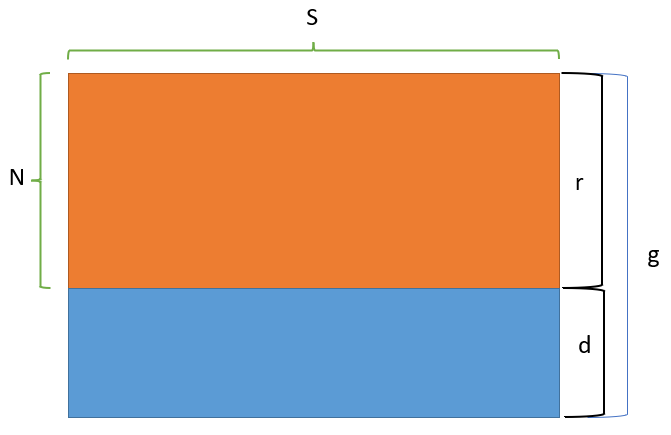
\includegraphics[width = 0.6\textwidth]{images/illu.png}
      \begin{itemize}
        \item $N$: the number of given lines. \quad $S$: the number of seats.
        \item $g$: total demand \quad $r$: remaining demand \quad $d$: discarded demand.
      \end{itemize}
    \end{frame}

    \begin{frame}{Formulation}
      \begin{itemize}
        \item Minimize the trim loss. $\min NS - \sum_{i=1}^m r_i(s_i-1) \to \max \sum_{i=1}^m r_i(s_i-1) \to \max \sum_{i=1}^m (g_i - d_i)(s_i-1)$.
        \item Recall that $\sum_{k=1}^K t_i^k x_k + d_i = g_i$, by substituting this equation we can obtain the objective function of the following master problem.
      \end{itemize}
      \[\begin{split}\mbox{max}\quad & \sum_{k=1}^K(\sum_{i=1}^m (s_i-1)t_i^k) x_{k}\\
      \mbox{s.t.} \quad & \sum_{k=1}^K x_{k} \leq N \\
      & \sum_{k=1}^K t_i^k x_k \leq g_i,\quad i=1,\ldots,m\\
      & x_{k} \geq 0, \quad k = 1,\ldots,K \\
      \end{split}\]
    \end{frame}

    \begin{frame}{Analysis}
      \begin{itemize}
        \item Similarly, we consider the linear relaxation of the master problem and the optimal dual variable vector $\lambda,\mu$.
        \item Using $\lambda$ as the value assigned to the first constraint and $\mu$ to the second constraints. The problem is to find a feasible pattern $(t_1^{k_0},t_2^{k_0},\ldots, t_m^{k_0})$ that maximizes the reduced cost.
        \item The reduced cost is $c_{k_0} - c_B B^{-1}A_{k_0}$, where $c_{k_0} = \sum_{i=1}^m (s_i-1)t_i^{k_0}, c_B B^{-1} = (\lambda,\mu)$, $A_{k_0} = (1,t_1^{k_0},t_2^{k_0},\ldots,t_m^{k_0})^T$.
        \item Use $y_i$ indicate the feasible pattern instead of $t_i^{k_0}$. We can obtain the sub-problem.
      \end{itemize}
    \end{frame}

    \begin{frame}{Sub-problem}
      \[\begin{split}\mbox{max}\quad & \sum_{i=1}^m \left[(s_i-1) -\mu_i\right] y_{i} - \lambda \\
      \mbox{s.t.} \quad & \sum_{i=1}^m s_i y_i \leq S  \\
      & y_i \geq 0, \mbox{integer}\quad \mbox{for}~ i=1,\ldots,m.\\\end{split}\]
      \begin{itemize}
        \item Use column generation to generate a new pattern until all reduced costs are negative.
      \end{itemize}
    \end{frame}

    \begin{frame}{IP Formulation}
      \[\begin{split}\mbox{max}\quad & \sum_{j=1}^{m} \sum_{i=1}^n (s_i-1) x_{ij} \\
      \mbox{s.t.} \quad & \sum_{i=1}^n s_i x_{ij} \leq S, \quad j=1,\ldots,m \\
      & \sum_{j=1}^{m} x_{ij} \leq g_i ,\quad i=1,\ldots,n \\
      & x_{ij} \geq 0 \mbox{ and integer}, \quad i=1,\ldots,n, j=1,\ldots,m \\\end{split}\]
      \begin{itemize}
        \item $m$ indicates the number of lines.
        \item $x_{ij}$ indicates the number of group type $i$ placed in each line $j$.
      \end{itemize}
    \end{frame}

    \begin{frame}{Improvement}
      \begin{itemize}
        \item For the cutting stock problem, $\min LP \leq \min LP^r \leq \min IP \leq \min IP^r$.
        After obtaining all patterns with column generation, restricted LP equals LP relaxation, $LP^r = LP$, which provides a lower bound. To obtain a optimal solution, we should implement branch and bound into column generation. This method is called branch-and-price.
        \item For the new problem, $\max LP \geq \max LP^r \geq \max IP \geq \max IP^r$. The column generation will give the upper bound (LP relaxation) and lower bound (restricted IP).
      \end{itemize}
    \end{frame}

    \begin{frame}{Branch scheme}
      \begin{itemize}
        \item General branch:
        $\sum_{k \in K\left(k^{j}\right)} x_{k} = \alpha$, where $K(p) = \{k \in K: k\geq p\}$ (column subsets) for $p \in Z^m_+$, $\alpha$ is fractional.
        $K = \{k \in N^m: \sum_{i=1}^m s_i k_i \leq S\}$ indicate all feasible patterns, and $x_k$ is the number of times pattern $k$ selected.
        \vspace{10pt}
        \item Given a feasible solution $x^*$ of LP that is not integral, take $k^*$ to be any maximal element of the set $\{k \in K: x_k^* \notin Z_+\}$. Then the only fractional term in this sum $\sum_{k \in K\left(k^{j}\right)} x_{k}^*$ is $x_{k^*}^*$.
        \vspace{10pt}
        \item Maximal means that the space left after cutting this pattern is less than the size of the smallest group.
      \end{itemize}
    \end{frame}

    \begin{frame}{Branch scheme}
      \begin{itemize}
        \item Generic branching constraints:
        $\sum_{k \in K(k^j)} x_{k} \leq U^{j}, \forall j \in G^u$ and $\sum_{k \in K(k^j)} x_{k} \geq L^{j}, \forall j \in H^u$,
        where $G^u$ and $H^u$ are sets of branching constraints of the form
        \begin{equation}
         \sum_{k \in {K(k)}} x_{k} \leq\lfloor\alpha\rfloor
        \end{equation} and
        \begin{equation}
        \sum_{k \in {K(k)}} x_{k} \geq \lceil\alpha\rceil
        \end{equation}, respectively.
        \vspace{10pt}
        \item If we can always generate the maximal pattern, then any fractional column defines a branching set which contains only one member.
        \vspace{10pt}
      \end{itemize}
    \end{frame}

    \begin{frame}{In our case}
      Restricted master problem:
      \[\begin{split}\mbox{max}\quad & \sum_{k\in K}(\sum_{i=1}^m (s_i-1)t_i^k) x_{k}\\
      \mbox{s.t.} \quad & \sum_{k \in K} x_{k} \leq N \\
      & \sum_{k \in K} t_i^k x_k \leq g_i,\quad i=1,\ldots,m\\
      & \sum_{k \in K(k^j)} x_{k} \leq U^{j}, \forall j \in G^u \\
      & \sum_{k \in K(k^j)} x_{k} \geq L^{j}, \forall j \in H^u \\
      & x_{k} \geq 0, \quad k \in K
      \end{split}\]
    \end{frame}

    \begin{frame}{In our case}
      Let $(\pi,\lambda,\mu,v)$ be optimal dual variables associated with the added constraints.
        The sub-problem is:

        \[\begin{split}\mbox{max}\quad & \left[(s_i-1) -\lambda_i\right] y_{i}- \pi - \sum_{j\in G^u}\mu_j z^j - \sum_{j\in H^u}v_j z^j \\
        \mbox{s.t.} \quad & \sum_{i=1}^m s_i y_i \leq S  \\
        & z^j =1 \mbox{ if } y \geq k^j; z^j =0 \mbox{ otherwise}  \\
        & y_i \geq 0, \mbox{integer}\quad \mbox{for}~ i=1,\ldots,m.
        \end{split}\]
        $Y_k = \{(y,z): z=1,\text{ if } y \geq k,z=0 \text{ otherwise} \}$ can be formulated as MIPs.
    \end{frame}

    \begin{frame}{In our case}
      \begin{itemize}
        \item The initial patterns are cut with as many copies as possible of each group size. To have the maximal patterns, just by adding as many copies as possible of the smallest group size.
        \item Our sub-problem is only affected when an upper bound has been placed on the value of the variable associated with the selected pattern. Because this variable could be a nonbasic variable for the LP. In this case, we have avoid regenerating this maximal pattern.
        \item Branch priority: select the least dominance pattern, and use the form(1). Because if we want to increase the total capacity, the number of low utilization pattern should be reduced.
      \end{itemize}
    \end{frame}

    \begin{frame}{Other branch-and-price methods}
      \begin{itemize}
        \item Transform the original sub-problem to 0-1 knapsack problem.
        \item Use DW decomposition. Less compact formulation.
        \item Use the definition directly. The subprobelm can be expressed as a MIP, not be a knapsack problem anymore.
      \end{itemize}
    \end{frame}

    \begin{frame}{Branch and Price}
        \begin{itemize}
          \item Solve restricted master problem with the initial columns.
          \item Use pricing problem to generate columns.
          \item When column generation terminates, is the solution integral?

          Yes, update lower bound.

          No, update upper bound. And fathom node or branch to create two nodes.
          \item Select the next node until all nodes are explored.
        \end{itemize}
    \end{frame}

    \begin{frame}{Properties}
      \begin{itemize}
        \item When column generation gives an integer solution at the first time, then we obtain the optimal solution.
        \item $\alpha_k$ indicates the number of items for pattern $k$. $\beta_k$ indicates the left space for maximal pattern $k$. Notice that the left space is the true loss.
        \item Denote $(\alpha_k + \beta_k)$ as the loss for pattern k, $l(k)$. When $l(k)$ reaches minimum, the corresponding pattern $k$ is the optimal solution for a single line.
        \item If the group sizes are consecutive integers starting from 2, $\{2,3,\ldots,u\}$, then a greedy-based pattern is optimal, i.e., select the maximal group size,$u$, as many as possible and the left space is occupied by the group with the corresponding size. The loss is $k+1$, where $k$ is the number of times $u$ selected. Let $S = u\cdot k + r$, when $r>0$, we will have at least $\lfloor \frac{r+u}{2} \rfloor -r +1$ optimal patterns with the same loss. When $r =0$, we have only one optimal pattern.
      \end{itemize}
    \end{frame}

    \begin{frame}
      \begin{itemize}
        \item Let $I_1$ be the set of patterns with the minimal loss. And $I_i$ be the set of patterns with $i$-th minimal loss.
        \item When supply is less than demand, we must select $I_1$.
        \item When $N \leq \max_{k\in I_1} \min_{i} \{\lfloor \frac{d_i}{b_i^k}\rfloor\}$, select the corresponding pattern from $I_1$ and it is the optimal solution.
        $N$ is the number of lines, $i = 1,2,\ldots, m$, $d_m$ is the demand of the largest size, $b_m^k$ is the number of group $m$ placed in pattern $k$.

      \end{itemize}
    \end{frame}

    \begin{frame}{Integral Decomposition}
      \begin{itemize}
        \item Denote by $R_+^n$ the nonnegative orthant of Euclidean n-space. A polyhedron $P \subset R_+^n$ is called lower comprehensive if $0 \leq y \leq x \in P$ implies $y \in P$.
        \item Let $M$ be the matrix whose rows are the maximal integral points of P.
        \item An integral vector $x \in P$ is a maximal integral point of $P$ if there is no integral vector $y \in P$ with $x \neq y \geq x$.
        \item Let $kP$ be defined as $\{kx|x \in P\}$.
        The integral decomposition property holds for
        $P$ if, for each integer $k \geq 1$ and each integral vector $x \in kP$, there exist integral vectors $x^i \in P, 1 \leq i \leq k$, for which $x = \sum_{i=1}^k x^i$.
        \item The knapsack polyhedron, denoted by $P$, is the convex hull of the set $\{x \in Z_+^n|ax \leq b\}$.
      \end{itemize}
    \end{frame}

    \begin{frame}{Integer Round Up for CSP}
      \begin{itemize}
        \item Cutting stock problem has the integer round-up property if and only if P has the integral decomposition property.
        \item Any two-dimension CSP has the IRU property.
        \item The numerical experiment shows that the form of $\{2,3,\ldots,n\}$ has the IRU property.
        \item But we can check this property finitely. From S. BAUM and L.E. TROTTER.
      \end{itemize}
    \end{frame}

    \begin{frame}{Integer Round Up for CSP}
      \begin{itemize}
        \item After the column generation gives the LP solution(fractional), calculate the supply quantity. If the number is integral, keep it.
        If the supply is not integral, we can construct an integer vector which can provide the largest integral profit.
        \item Construction: Calculate the space taken by fractional supply(the value must be integer), increase the corresponding supply having the same space, delete the fractional part.
        \item Now we have an integral supply vector. If this case has IRU property, there exists an integral decomposition.
        \item Minus the integral part of the patterns from the supply. Check if the rest can be placed in several lines.
      \end{itemize}
    \end{frame}

    \begin{frame}{Need to do}
      \begin{itemize}
        \item If the left space is 1? solved.
        \item If the left, subset sum problem.
        \item Check when L = 22
      \end{itemize}

    \end{frame}


    \begin{frame}{}
      Reformulate our model as:
      \[\begin{split}\mbox{max}\quad & yMc \\
      \mbox{s.t.} \quad & yM \leq w_0 \\
      & \sum y \leq N \\
      & y \geq 0 \mbox{ and integer} \end{split}\]

      $w_0$ is the demand. $N$ is the number of given lines.
    \end{frame}

    \begin{frame}{}
      \[\begin{split}\mbox{min}\quad & \sum y \\
      \mbox{s.t.} \quad & yM \geq w \\
      & y \geq 0 \mbox{ and integer}\end{split}\]

      \[\begin{split}\mbox{max}\quad & c w \\
      \mbox{s.t.} \quad & w \in \{Nx| x \in P\} \\
      & w \leq w_0\end{split}\]

      When P has the integral decomposition property, there exist $N$ integer vectors decomposing every $w$.
      Now, the question is how to find the maximal $w$.
    \end{frame}

    \begin{frame}{Question}
      \begin{itemize}
        \item Which patterns will be covered?
        \item Only select $I_1$, demand has to satisfy which condition?
        \item We only need $I_1$ and $I_2$ when supply and demand?
      \end{itemize}
    \end{frame}

    \begin{frame}{Lower Bound for Demand}
      \[\begin{split}\mbox{max}\quad & \sum_{k=1}^K(\sum_{i=1}^m (s_i-1)t_i^k) x_{k}\\
      \mbox{s.t.} \quad & \sum_{k=1}^K x_{k} \leq N \\
      & \sum_{k=1}^K t_i^k x_k \leq g_i,\quad i=1,\ldots,m\\
      & \sum_{k=1}^K t_i^k x_k \geq p_i,\quad i=1,\ldots,m\\
      & x_{k} \geq 0, \quad k = 1,\ldots,K \\
      \end{split}\]
      \begin{itemize}
        \item Use the similar method to solve.
      \end{itemize}
    \end{frame}

    \begin{frame}{Sub-problem}
      \[\begin{split}\mbox{max}\quad & \sum_{i=1}^m \left[(s_i-1) -\lambda_i - \mu_i \right] y_{i} - \tau \\
      \mbox{s.t.} \quad & \sum_{i=1}^m s_i y_i \leq S  \\
      & y_i \geq 0, \mbox{integer}\quad \mbox{for}~ i=1,\ldots,m.\\\end{split}\]
      \begin{itemize}
        \item Use column generation to generate a new pattern until all reduced costs are negative.
      \end{itemize}
    \end{frame}

    \begin{frame}{IP Formulation}
      \[\begin{split}\mbox{max}\quad & \sum_{j=1}^{m} \sum_{i=1}^n (s_i-1) x_{ij} \\
      \mbox{s.t.} \quad & \sum_{i=1}^n s_i x_{ij} \leq S, \quad j=1,\ldots,m \\
      & p_i \leq \sum_{j=1}^{m} x_{ij} \leq g_i ,\quad i=1,\ldots,n \\
      & x_{ij} \geq 0 \mbox{ and integer}, \quad i=1,\ldots,n, j=1,\ldots,m \\\end{split}\]
      \begin{itemize}
        \item $m$ indicates the number of lines.
        \item $x_{ij}$ indicates the number of group type $i$ placed in each line $j$.
      \end{itemize}
    \end{frame}

    \begin{frame}{Question}
        1. Feasibility. At first, use cutting stock model to check if the following constraints provide a feasible solution. If the minimal number of lines we need is less than the given number of lines, these constraints are feasible.
        \[\begin{split}
        & \sum_{i=1}^n s_i x_{ij} \leq S, \quad j=1,\ldots,m \\
        & p_i \leq \sum_{j=1}^{m} x_{ij},\quad i=1,\ldots,n
        \end{split}\]

    \end{frame}


    % \begin{frame}{Extension}
    %
    % \end{frame}
